\chapter{Accretion Disc Winds}
\label{sec:winds}

\epigraph{``A view of space, with an elephant obstructing it"}
{{\sl Mike Vennart, Silent/Transparent}}


%%%%WINDS 
%%% COULD MAKE THIS A NEW CHAPTER
\section{Accretion Disc Winds: Observational Evidence}

\subsection{Cataclysmic Variables}



\subsection{X-ray Binaries}
\label{sec:xrb_winds}




\subsection{AGN and Quasars}

\subsubsection{Broad Absorption Line Quasars}

\subsubsection{Warm Absorbers}

\subsubsection{Ultra-fast Outflows}




\subsection{Stellar Winds}

\subsubsection{Clumping}

\section{Accretion Disc Winds: Driving Mechanisms}

Let us consider a parcel of ideal gas. By imposing nothing more than
conservation of mass, energy and momentum on that parcel we can write down
three equations of hydrodynamics
\footnote{I stress that these equations are not used in hydrodynamic
simulations in this thesis (see section ?, for example); 
they are discussed here because they provide a natural reference point
for exploring potential driving mechanisms for winds in accreting systems.
}

\begin{equation}
\label{eq:continuity}
\frac{D \rho}{Dt} + \rho \nabla \cdot \vec{v} = 0
\end{equation}

\begin{equation}
\label{eq:motion}
\rho \frac{Dv}{Dt} = -\nabla P + \frac{1}{4 \pi}(\nabla \times \vec{B}) \times \vec{B} + \rho \vec{F}_{rad} + \rho \vec{g}
\end{equation}

\begin{equation}
\label{eq:energy}
\rho \frac{D}{Dt} \left(\frac{e}{\rho}\right) = P \nabla \cdot \vec{v} + \rho \cal{L}
\end{equation}

Here $D$ denotes a derivative within the comoving frame of the gas parcel, $\vec{v}$ is the velocity,
$\rho$ is the gas density, $\vec{B}$ is the local magnetic field, $\vec{F}_{rad}$ is the radiation
force per unit mass and $\vec{g}$ denotes the gravitational acceleration vector.
Equation~\ref{eq:continuity} is the {\em continuity equation} and describes conservation of mass. 
Equation~\ref{eq:motion} is the {\em equation of motion} and describes conservation of momentum.
Equation~\ref{eq:energy} is the {\em equation of energy conservation}. 
We can use equation~\ref{eq:motion} to neatly demonstrate how an outflow can be driven. I have 
deliberately written the equation so that all the force terms lie on the RHS. We can then see that
for an outflow to be driven from an accreting object one simply needs one of the terms on
the RHS to dominate over gravity, $\rho \vec{g}$. These terms thus signify three potential
driving mechanisms.

\begin{itemize}
	\item Magnetic Forces, $\frac{1}{4 \pi}(\nabla \times \vec{B}) \times \vec{B}$.
	\item Radiative Forces, $\rho \vec{F}_{rad}$.
	\item Thermal Pressure, $-\nabla P$.
\end{itemize}

We can now examine under what physical conditions (and in which corresponding astrophysical objects)
we might expect these forces to overcome gravity and cause a parcel of mass to escape to infinity.
In other words: {\em what might drive a wind?}

\subsection{Thermal Winds}

In hydrostatic equilibrium (HSE), thermal pressure balances gravity and no other forces 
are present, meaning that the equation of motion can be written as 
\begin{equation}
\label{eq:hse}
\rho \frac{Dv}{Dt} = -\nabla P +  \rho \vec{g} = 0
\end{equation}
Clearly, if the thermal pressure is then significantly 
increased then this equilibrium condition no longer holds. 
This can occur in accretion discs at temperatures in excess of $\sim10^7$~K --
where other forces are negligible compared to thermal pressure -- 
and where the escape velocities are relatively low (i.e. far out in the disc).
Due to the temperature and gravity scalings, this means
that XRBs are natural candidates for showing evidence of thermally driven
winds. The outer disc can be heated to the Compton temperature by the central X-ray source,
potentially driving relatively high mass-loss rate outflows \citep{begelman1983,woods1996}. 
This driving mechanism has been proposed as a natural explanation
for the ever-present equatorial outflows in soft state XRBs \citep{ponti2012}.
However, they are much less likely candidates in CVs and AGN {\bf Discuss scaling
arguments with equations?}.


\subsection{Radiatively Driven Winds}

\subsection{Line-driven Winds}

\subsection{Magneto-centrifugal Winds}

\section{Accretion Disc Wind Models}


\section{A Kinematic Prescription}




\section{The really, really big picture: AGN Feedback}

The event horizon of a $10^9~M_\odot$ BH is approximately 
$10^{15}$~cm, a billionth of the size of a typical galactic bulge. This is 
roughly the difference in size between a small coin and the radius of the 
Earth. Despite this vast different in scale, there are multiple
pieces of evidence that the physics on the scale of the gravitational
radius of the BH really does affect the evolution and dynamics of its host galaxy.
I shall briefly discuss the evidence for this statement, and 
assess the potential role of winds together with alternative mechanisms.

\subsection{Observational evidence for feedback}

Perhaps the most famous pieces of evidence for some kind of long-distance 
relationship between a central BH and its host galaxy are the 
$M_{BH}-\sigma_*$ and $M_{BH}-M_{bulge}$ correlations, shown in figures~\ref{fig:msigma}
and \ref{fig:mbulge} respectively.

\nocite{mcconnell2013,gultekin2009}
\begin{figure}
\centering
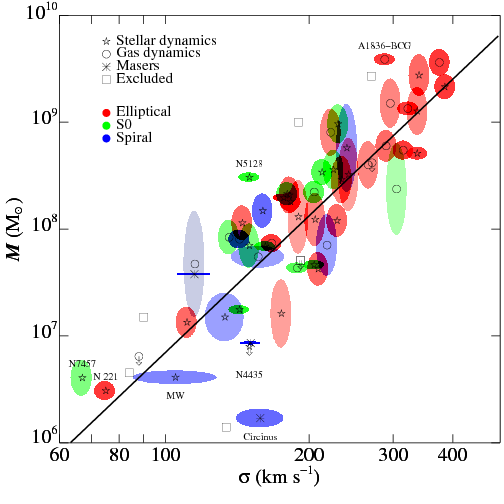
\includegraphics[width=0.7\textwidth]{figures/02-outflows/msigma.png}
\caption
{
{\sl Credit: Gultekin et al. 2009}. 
The $M_{BH}-\sigma_*$ correlation.
} 
\label{fig:mbulge}
\end{figure}

\begin{figure}
\centering
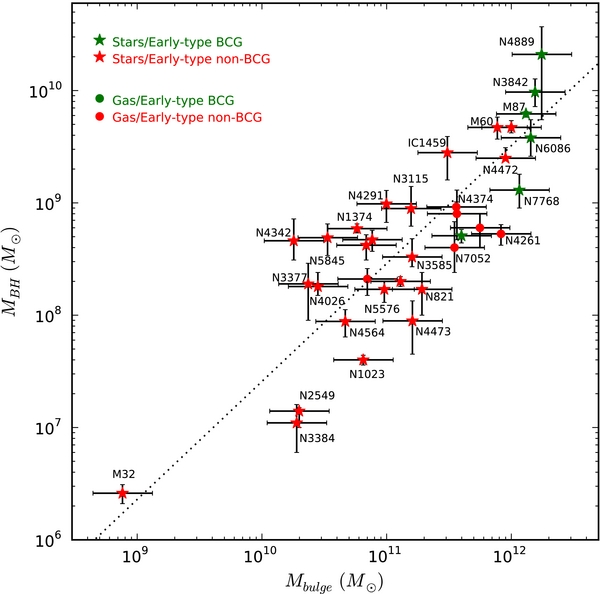
\includegraphics[width=0.7\textwidth]{figures/02-outflows/mbulge.jpg}
\caption
{
{\sl Credit: McConell \& Ma 2013}. 
The $M_{BH}-M_{bulge}$ correlation.
} 
\label{fig:mbulge}
\end{figure}

\subsection{Radiative or quasar mode feedback}

\subsection{Kinetic or radio mode feedback}

\subsection{In-situ Explanations}


